\documentclass{article}
\usepackage[utf8]{inputenc}
\usepackage[spanish]{babel}
\usepackage{listings}
\usepackage{graphicx}
\graphicspath{ {images/} }
\usepackage{cite}

\begin{document}

\begin{titlepage}
    \begin{center}
        \vspace*{1cm}
            
        \Huge
        \textbf{Informe}
            
        \vspace{0.5cm}
        \LARGE
        Solucion del desafio
            
        \vspace{1.5cm}
            
        \textbf{Jhonny Alejandro Ortiz Osorio}
            
        \vfill
            
        \vspace{0.8cm}
            
        \Large
        Despartamento de Ingeniería Electrónica y Telecomunicaciones\\
        Universidad de Antioquia\\
        Medellín\\
        Marzo de 2021
            
    \end{center}
\end{titlepage}

\tableofcontents
\newpage
\section{Descripción de la actividad}\label{intro}
Esta actividad consiste en describir una seria de pasos donde se llevará un objeto desde un estado inicial A hasta un estado final B, se pondrá a prueba con 3 personas diferentes que lo único que sabrán es que deben de seguir una serie de pasos anteriormente mencionados.

\section{Pasos para realizar el desafío} \label{contenido}
\begin{figure}[h]
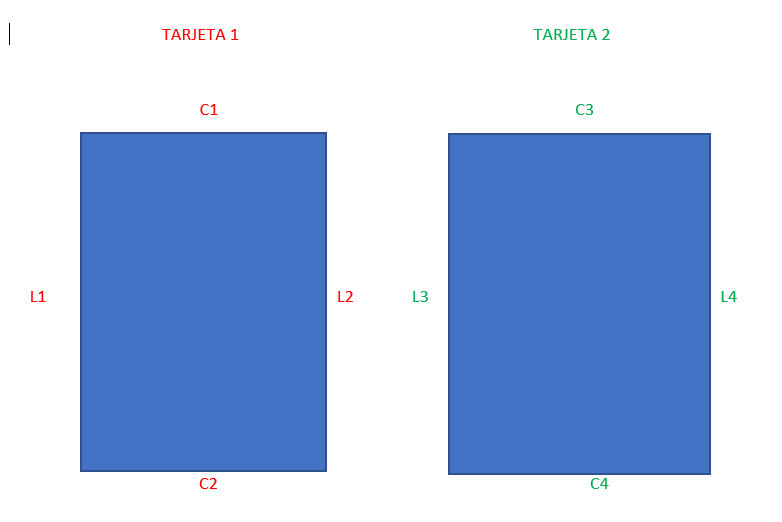
\includegraphics[width=15cm]{Tarjetas.png}
\centering
\caption{Nombre de las tarjetas y sus lados}
\label{fig:tar}
\end{figure}

\textbf{ESTADO INICIAL} \\\\
Dos tarjetas unidas encima de una mesa y una hoja de papel totalmente en blanco cubriendo las tarjetas. \\\\
\textbf{PASO 1} \\\\
Tomar la hoja con la mano derecha por una esquina con mucha precaución de no hacerle ningún daño a la hoja y levantarla hasta que ya no tape las tarjetas. \\\\
\textbf{PASO 2} \\\\
Colocar la hoja sobre la mesa, procurando que no quede encima de las tarjetas. \\\\
\textbf{PASO 3} \\\\
Mirar la figura \ref{fig:tar} donde se nombran las tarjetas y cada uno de sus lados, siendo la tarjeta de abajo la numero 1 (con lados: L1, L2, C1, C2) y la de arriba la numero 2 (con lados: L3, L4, C3, C4). Los lados L1, L3 están juntos, los lados L2, L4 están juntos, los lados C1, C3 están juntos y los lados C2, C4 están juntos. \\\\
\textbf{PASO 4} \\\\
Tomar las tarjetas con la mano derecha colocando el dedo pulgar en los lados L1, L3 presionando suavemente hacia el lado contrario y los dedos índice, medio y anular en los lados L2 y L4 presionando suavemente hacia el lado contrario. \\\\
\textbf{PASO 5} \\\\
Colocar las tarjetas, sin soltarlas de la mano derecha, sobre la hoja por los lados C2 Y C4, procurando que los lados C1, C3 apunten hacia el techo. \\\\
\textbf{PASO 6} \\\\
Posicionar los dedos de la mano derecha con base a las siguientes instrucciones: el dedo índice se apoyará en los lados C1 y C3, los dedos medio y anular se posicionarán en el lado L4 y el dedo pulgar se posicionará en el lado L3. \\\\
\textbf{PASO 7} \\\\
Sin soltar las tarjetas, alejar los lados L3 y L4 de los lados L1 y L2, hasta formar una pirámide con las dos tarjetas. \\\\
\textbf{PASO 8} \\\\
Retirar la mano derecha con mucha precaución intentando que las dos tarjetas se sostengan por sí solas. \\\\
\textbf{EN CASO DE QUE LAS TARJETAS NO SE SOSTEGAN POR SI SOLAS} \\\\
\\\\
\textbf{PASO 9} \\\\
Colocar la tarjeta 2 encima de la tarjeta 1 de manera que los lados L1, L3 queden juntos y los lados C1, C3 también queden juntos. \\\\
\textbf{PASO 10} \\\\
Volver al \textbf{PASO 4} y repetir el proceso hasta lograr con éxito el \textbf{PASO 8}.

\end{document}
